\documentclass[conference]{IEEEtran}

\makeatletter
\newcommand{\rmnum}[1]{\romannumeral #1}
\newcommand{\Rmnum}[1]{\expandafter\@slowromancap\romannumeral #1@}
\makeatother

\usepackage{cite}
\usepackage{amsmath}

\ifCLASSINFOpdf
   \usepackage[pdftex]{graphicx}
  % declare the path(s) where your graphic files are
   \graphicspath{{./png/}}
  % and their extensions so you won't have to specify these with
  % every instance of \includegraphics
   \DeclareGraphicsExtensions{.pdf,.png}
\else
  % or other class option (dvipsone, dvipdf, if not using dvips). graphicx
  % will default to the driver specified in the system graphics.cfg if no
  % driver is specified.
  % \usepackage[dvips]{graphicx}
  % declare the path(s) where your graphic files are
  % \graphicspath{{../eps/}}
  % and their extensions so you won't have to specify these with
  % every instance of \includegraphics
  % \DeclareGraphicsExtensions{.eps}
\fi

\ifCLASSOPTIONcompsoc
    \usepackage[caption=false,font=normalsize,labelfont=sf,textfont=sf]{subfig}
\else
    \usepackage[caption=false,font=footnotesize]{subfig}
\fi

    

% correct bad hyphenation here
\hyphenation{op-tical net-works semi-conduc-tor}
\newcommand{\ignore}[1]{{}}

\begin{document}

\title{Robust Energy-Aware Routing with Uncertain Traffic Demands}


\author{\IEEEauthorblockN{Heng Lin}
\IEEEauthorblockA{Tsinghua University \\ henglin1991@gmail.com}
\and
\IEEEauthorblockN{Mingwei Xu}
\IEEEauthorblockA{Tsinghua University \\ xmw@cernet.edu.cn}
\and
\IEEEauthorblockN{Yuan Yang}
\IEEEauthorblockA{Tsinghua University \\ yyang@csnet1.cs.tsinghua.edu.cn}}


% make the title area
\maketitle

% As a general rule, do not put math, special symbols or citations
% in the abstract
\begin{abstract}
Energy conservation has become a major challenge to the Internet. In existing approaches, a part of line cards
are switched into sleep mode for energy conservation, and the routing is configured carefully to balance energy saving
and traffic engineering goals, such as the maximum link utilization ratio (MLUR). Typically, traffic demands are
used as inputs, and routing is computed accordingly. However, accurate traffic matrices are difficult to obtain and
are changing frequently. This makes the approaches difficult to implement. Further, the routing may shift
frequently, and is not robust to sudden traffic changes.

In this paper, we propose a different approach that finds one energy-aware routing robust to a set of traffic
matrices, particularly to arbitrary traffic demands. Such a routing without energy consideration is known as
the demand-oblivious routing, and is well studied. However, the problem becomes much more challenging when energy
conservation is involved. To overcome the challenges, we first define a new metric, namely oblivious performance
ratio (OPR) with energy constraint, which reflects the MLUR distance from a routing to the optimal routing when
certain energy conservation requirement is satisfied. We model the problem of minimizing the performance ratio,
and analyze the lower and the upper bounds. Then, we propose Robust Energy-Aware Routing (REAR) to solve
the problem in two phases. REAR select sleeping links based on extended robust link utilization (ERLU) or algebraic
connectivity, and compute the routing based on a classical demand-oblivious routing algorithm.
We evaluate our algorithms on real and synthetic topologies. The simulation results show that REAR can save
19\% of line card power while the performance ratio is less than 34\%.
\end{abstract}

\IEEEpeerreviewmaketitle

\section{Introduction}

Energy conservation has become a global concern nowadays. The Internet is one of the major energy consumers, and its rapid growth makes the green Internet a hot research topic. In the Internet backbone, energy is mainly drawn by routers and switches. Such devices consume almost full power even if the traffic load is small. Thus, an effective method to save energy in the Internet is to aggregate traffic into part of the routers when the traffic load is small, and switch the under-utilized components (routers or line cards) into off/sleep mode. Such a method is known as the energy efficient routing.

An important issue for energy efficient routing is to avoid network congestion after the traffic is aggregated. Many approaches have been proposed in existing works. Most approaches compute the routing based on real-time traffic matrices or link loads, to achieve a good load balancing and avoid congestion. However, such approaches come at a cost of obtaining real-time traffic data. Furthermore, the routing may shift frequently with the traffic changes, and a sudden traffic change may still induce congestions. To this end, we need to study the robustness of energy efficient routing.

Specifically, we study the energy efficient routing when traffic matrices cannot be obtained or predicted precisely, i.e., with uncertain traffic demands. To achieve robustness, we need to find a routing, which can perform near optimally under a range of traffic matrices. The key technique that makes this possible is the advanced \emph{demand-oblivious routing}. A seminal work \cite{networking:oblivious} find that, the distance between the maximum link utilization ratio (MLUR) of a demand-oblivious routing and the MLUR of the optimal routing is bounded. Thus, no matter how the traffic demand changes, the demand-oblivious routing can guarantee certain performance. We note that this conclusion is in a network without off/sleep components, and we need to consider the situation when energy conservation is required.

However, existing demand-oblivious routing algorithms cannot be directly applied to energy efficient routing. There are several challenges. First, we need to define a metric that can effectively measure the distance between a robust energy efficient routing and the optimal routing, because the existing metric for demand-oblivious routing fails in the situation when some components are switched into off/sleep mode. Second, we need to analyze whether the metric can be bounded, just like for demand-oblivious routing. If there exists no bound, then it is not feasible to find a robust energy efficient routing. Third, we need practical algorithms to compute the robust energy efficient routing. Specifically, we need to determine: 1) which routers or line cards should be switched into off/sleep mode, to achieve energy efficiency; and 2) in which path to forward the traffic for robustness, while the path does not traverse the off/sleep components.

In this paper, we overcome the aforementioned challenges. First, we define a new metric, namely the oblivious performance ratio with energy constraint (OPRE). The OPRE reflects the MLUR distance from a routing to the optimal one when certain energy conservation requirement is satisfied. We model the problem of minimizing the OPRE. Second, we prove that there exists a robust energy efficient routing with the minimum OPRE, which has an upper bound given a network. Then, we propose Robust Energy-Aware Routing (REAR) scheme, which uses heuristic algorithms to solve the problem. We develop algorithm XXX, which chooses off/sleep line cards in a way that the OPRE can be minimized potentially. We then develop algorithm XXX to compute the routing in the remaining topology, by extending existing optimal demand-oblivious routing algorithm. We evaluate our algorithms by simulations on real topologies and synthetic traffic demands with random fluctuations. The results show that REAR can achieve an OPRE of 1.34 while 19\% of line card power is saved.

The rest of the paper is organized as follows. Section \Rmnum{2} shows the related work. Section \Rmnum{3} presents metric OPRE and formally models the problem. We presents the bounds on OPRE in Section \Rmnum{4}, and propose our algorithms in Section \Rmnum{5}. Section \Rmnum{6} shows our simulation setup and results, and Section \Rmnum{7} concludes our work.

\ignore{
Usually, We compute routing to stipulate how is the traffic going, to achieve some traffic engineering goals such as
the maximum link utilization ratio (MLUR). In details, we use traffic demands and network topology as input for
computation, then combine routing and traffic demands to get the traffic on each link, based on which we determind
which link can be put to sleep. However, measuring and predicting accurate traffic demands are difficult, so does its dynamic
natrue. Although we have obtained all knowledge about traffic demands, the corresponding routing may shift frequently
when the traffic demands change. It means that we should change the link (line cards) working mode frequently as well,
of course it is unpractical. So we need the routing be robust to sudden traffic changes, and based on the approximate traffic demands.
Such a routing is known as the demand-oblivious routing and is well studied in \cite{networking:oblivious}, which proposes
the algorithm for computing robust routing with uncertain traffic demands on specific topology.


Unfortunately, there is no metric in such robust routing to measure the importance of links, in another word, we have no
idea to put which link to sleep mode. Furthermore, when some links are switched off and the topology changed actually, but we
still have no idea for how to adjust the routing in result topology. Another challenge is that, to achieve the power saving
goals we may should switch off not only one link, and it is a classical NP-Hard problem. To overcome the challenges,
we define a metric namely extended robust link utilization (ERLU) to measure the traffic engineering natrue of link without real traffic
demands, and define oblivious performance ratio (OPR) to reflect the MLUR distance from a routing to the optimal one
when certain energy conservation requirement is satisfied. In our algorithm, we use algebraic connectivity \cite{networking:algebraic} and
ERLU as criterion to switch off links, and use OPR to adjust routing.


Our main contribution in this paper is three-fold. Firstly, we model the problem of minimizing the OPR, then
analyze the lower and the upper bounds. Secondly, we propose an heuristic algorithm named Robust Energy-Aware Routing (REAR)
to solve the problem in two phases, includes choosing links to sleep and adjusting routing. Thirdly, we implement our
algorithm on real topology and arbitrary traffic demands to observe the relationship between energy conservation and OPR. The
simulation results show that REAR can save 19\% power of line cards while OPR is less than 34\% in some topology. Also
we investigate the path stretching problem.


The rest of the paper is organized as follows. Section \Rmnum{2} reviews the related work and Section \Rmnum{3}
defines two metric and models our problem. Following we propose our algorithm in Section \Rmnum{4}. For clearer understanding
on our problem, we give two simple samples and prove the bounds in Section \Rmnum{5}. Experiments are discribed
and result are showed in Section \Rmnum{6}. We discuss issues and future work in Section \Rmnum{7}, then conclude our wok in
Section \Rmnum{8}}

\section{Related Work}
related work

\section{Problem Statement}

\subsection{Background of Demand-Oblivious Routing}

As mentioned above, demand-oblivious routing aims at finding one routing that performs near optimally under a range of traffic demands. In traffic engineering, a typical metric to evaluate routing performance is the maximum link utilization ratio (MLUR). Clearly, the MLUR is corresponded with a specified traffic matrix (TM). Demand-oblivious routing defines oblivious performance ratio (OPR) to evaluate the routing performance without the knowledge of TM. We briefly present the background.

Given a TM, the distance between a routing to the optimal one is defined as the ratio between their MLURs. Formally, a network is modeled as undirected graph $G(V, E)$, where $V$ is the set of vertices (nodes), and $E$ is the set of edges (links). Let $cap_{ij}$ denote the capacity of the link $(i, j) \in E$. Let $d_{ab}$ denote the traffic demand from origin node $a$ and destination node $b$, and $m$ denote the TM that contains $d_{ab}$ for all $a, b \in V$. Let $f_{ab}(i,j)$ be the fraction of $d_{ab}$ that is routed on link $(i, j)$ $(0 \leq f_{ab}(i,j) \leq 1)$. Routing $r$ is specified by $f_{ab}(i,j)$ for all $a, b \in V$ and $(i, j) \in E$, and we will formally define routing consistency later in Section III.C. Let $U_{r, m, G}$ be the MLUR of routing $r$ under TM $m$. We have
\begin{equation}
	U_{r, m, G} = \max_{(i,j)\in E} \frac{\sum_{a,b} d_{ab}f_{ab}(i,j)}{cap_{ij}}.
\end{equation}
Let $P(\{ r \},\{ m \}, G)$ be the \emph{performance ratio} of routing $r$ under TM $m$, which reflects how far from the routing to the optimal one, and is defined as
\begin{equation}
	P(\{ r \},\{ m \}, G) = \frac{U_{r,m,G}}{\min_{r'} U_{r', m, G}}.
\end{equation}

The \emph{oblivious performance ratio} (OPR) for routing $r$ is defined by extending TM $m$ to a set of TMs $M$, where $M$ can be the set of any TMs. We have
\begin{equation}
	P(\{ r \}, M, G) = \max_{m\in M} P(\{ r \}, \{ m \}, G).
\end{equation}
The target of demand-oblivious routing is to find routing $r$ that minimizes OPR $P(\{ r \}, M, G)$. Such a ``robust'' routing is independent of a specific TM, but can perform near optimally. A seminal work \cite{networking:oblivious} uses linear programming to find the routing that minimizes the OPR, and finds that the optimal solution exists, which means that the OPR is bounded.

\subsection{Oblivious Performance Ratio with Energy Constraint}

With energy constraint, a network may have to switch part of line cards into off/sleep mode to save the total energy consumption. This changes the network topology and makes metric OPR fail to evaluate the robustness of a routing. We use an example to show this. Assume that $G$ is a cycle with $n$ unit capacity links. Then, the minimal OPR of $G$ is $2-2/n$ \cite{networking:oblivious}. Now we pruning one link from $G$ to save energy, and the topology changes to $G^*$. Because there is only one routing feasible in $G^*$, OPR $P(\{ r \}, M, G^*)$ equals 1. Since 1 is less than $2-2/n$ for $n > 2$, it means that the routing after pruning one link is more robust than before. However, it is false because there are less links and the network is more likely to be congested.

The intrinsic reason for such a ``fake robust'' is that the topology is not changing when performance ratio is computed in Eq. (2). To address this issue, we extend the definition of OPR. Formally, let $G^*$ be a sub-graph of $G$ that satisfies the energy constraint (We will formally give the model in Section III.C). The extended performance ratio is defined as
\begin{equation}
	P(\{ r \},\{ m \}, G, G^*) = \frac{U_{r,m,G^*}}{\min_{r'} U_{r', m, G}}.
\end{equation}
Let $P^*(\{ r \}, M, G)$ be the \emph{oblivious performance ratio with energy constraint} (OPRE) for routing $r$. We define $P^*(\{ r \}, M, G)$ by extending $m$ to $M$, and finding $G^*$ that satisfies the energy constraint and has the minimum performance ratio. We have
\begin{equation}
	P^*(\{ r \}, M, G) = \min_{G^*} \max_{m\in M} P(\{ r \}, \{ m \}, G, G^*)
\end{equation}
Note that when there is no energy constraint, $G$ is the sub-graph that has the minimum performance ratio, and Eq. (5) naturally reduces to Eq. (3).

\subsection{Problem Formulation}
We formulate our problem as following:

\begin{equation}
Minimize \max_{m \in M} \frac{U_{r,m,G^*}} {min_{r'} U_{r', m, G}}
\end{equation}

\begin{equation}
    G^* = (V,E^*), E^* \subset E
\end{equation}

\begin{equation}
    \begin{split}
    \forall (\epsilon, \gamma) \in \{ (E, r'), (E^*, r)\} \\
    \sum_{(i,j) \in \epsilon}f_{ab}(i,j)O_{(i,j)}^i - \sum_{(i,j) \in \epsilon}f_{ab}(i,j)I_{(i,j)}^i = \\
    \left\{
        \begin{array}{c}
        1, i = b \\
        -1, i = a \\
        0, i \neq a,b \\
        \end{array}
    \right.
    , \ \ \ \ a,b,i \in V, a \neq b, f_{ab}(i,j) \in \gamma
    \end{split}
\end{equation}

\begin{equation}
    \sum_{l \in E^*} p(l) / \sum_{l \in E} p(l) < 1 - \theta
\end{equation}

Eq. (6) is our target, which minimize the value of OPRE defined in \Rmnum{3}.B. Eq. (7) say $G^*$ be a sub-graph of $G$, which means remove/sleep
some links from $G$, and keep vertices the same. Eq. (8) ensures the graph is connected and define the routing. In details, $O_{(i,j)}^i$ equal to
1 if $i$ is the tail node of link $(i,j)$, and $I_(i,j)^i$ equal to 1 if $i$ is the head node of link $(i,j)$, this equation states the flow 
conservation constraints. In the other hand, $f_{ab}(i,j)$ is specified by routing $\gamma$, if the graph is not connected it will be unavailable
for some origin and destination pair. And from Eq. (8) we know that routing $r$ is corresponded with $G^*$, and $r'$ with $G$. We calculate the 
power constraints in Eq. (9), it ensure that we can save more than $\theta$ energy consumption. The function $p$ which maps link to power consumption
is proposed in \cite{networking:greente}.

\subsection{Model Example}
We will take an example to explain how to choose the link to close in our algorithm.
Three hostes include : a, b, c, three links are with repectively capacity of 3M, 4M and 2M. For simpleness, we suppose
there are two TM : ${(a,b,2M), (a,c,1M)}$ and ${(a,b,1M), (a,c,1M)}$. For each traffic matrix, the optimal route is
obvious, we will trace 2M from a to b across the lower link and trace the 1M from a to c across the upper one
for the first traffic matrix, whose maximum link utilization is 0.5. we will trace all the traffic acorss the
lower link for the second traffic matrix, whose maximum link utilization is 0.5 as well.


\begin{figure}[!t]
\centering
\vspace*{0.1in}
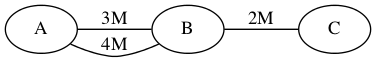
\includegraphics[width=8cm]{3-nodes-example}
\caption{Model Example, TM \Rmnum{1} : (a, b, 2M), (a, c, 1M); TM \Rmnum{2} : (a, b, 1M), (a, c, 1M).}
\label{label}
\vspace*{0.1in}
\end{figure}


Now for some reason, we will choose one link to shut down for power saving without lose connection of the network.
There are two choice, remove either the upper link or the lower link. Let us take a little calculation: when
remove the upper one, we should change all the traffic acorss the lower link, as a result, in the first
TM the maximum link utilization is 0.75 and the second is 0.5; when close the lower link, we should trace all the
traffic acorss the upper link, in the first TM the link utilization is 1 and the other is 0.667.
So according to our theory, the $P^{*}(M, G)$ should be 1.5 and the optimal successor network topology will be
the one which 3M link is closed.

\section{Algorithm}
In our paper, Robust Energy-Aware Routing (REAR) algorithm works in two phases. Firstly, REAR select links 
should be put to sleep from the origin topology based on extended robust link utilization or algebraic connectivity, 
then compute the robust routing by demand-oblivious routing algorithm. There are two metrics
for selecting removed links, our two-phase algorithm is flexible because we can replace the metric with whatever
metric.


\subsection{Algebraic Connectivity}
Network topology is represented by $G = (V, E)$ as mentioned in Model section, where $V$ is the set of vertices
and $E$ is the set of links. We say $A(G)$ is the Adjacency Matrix of graph $G$, that include information for which
vertices of the graph are adjacent to which other vertices. $A(G)$ is a $N \times N$ matrix, where
$N = |V|$ and non-diagonal entry $a_{ij}$ equal to the number of edges from vertex $i$ to vertex $j$, in this paper,
$a_{ij}$ always be 1 if $(i,j) \in E$ otherwise 0. And we stipulate the diagonal element $a_{ii}$ be 0.


We say $D(G)$ is the Degree Matrix of graph $G$, which is a diagonal matrix and diagonal entry $d_{ii}$ denote 
the degree of node $i$. It is obvious that there is $d_{ii} == \sum_{j} a_{ij}$.


Then we define Laplacian Matrix $L(G)$ of graph $G$ as the difference between Degree Matrix and Adjacency Matrix :
\begin{equation}
	L(G) = D(G) - A(G)
\end{equation}
where $D(G)$ is the Degree Matrix and $A(G)$ is the Adjacency Matrix.


In the mathematical field of graph theory, the number of eigenvalues equal to 0 is the number of connected 
componements of $G$, so the smallest eigenvalue always be 0 in arbitrary graph . And we call the second smallest one as
algebraic connectivity, which is greater than 0 if and only if graph $G$ is connected. Further more,  
it measures the connectivity and stability of graph, the greater of the value, the more connective of graph;
and it is a metric of average distance between any two vertices of graph $G$. We call the algebraic connectivity as
$\lambda_2(G)$.


Topology always have different algebraic connectivity values, it is clear that when one link is added or 
removed from the graph, the algebraic connectivity value changes accordingly. And we say the changed value
is the impact of this link on the graph. Supposed we sleep link $l$ from graph $G$, new graph is described as $G^*$, 
we defined the impact of link $l$ as :
\begin{equation}
	\Delta_l = \lambda_2(G) - \lambda_2(G^*)
\end{equation}
where $\lambda_2(G)$ and $\lambda_2(G^*)$ is algebraic connectivity of $G$ and $G^*$ respectly.


Clearly, $\Delta_l$ is always greater than 0, because graph will always lose connectivity when link is removed.
Further more, some link will play a more important role in the connectivity of graph, such as the backbone link 
of network topology. And we say a link $l$ affect more if $\Delta_l$ is greater.

\subsection{Extended Robust Link Utilization}
The demand-oblivious routing is not always the best one for 
specific $TM$, but good enough for a range of $TM$. we mentioned the definition of link utilization above when 
demand and routing are determined, as demand become oblivious, the definition is also not suitable. So we define
a notation named extended robust link utilization (ERLU) replace the normal link utilization like :
\begin{equation}
	u^e_{ij} = \frac {\sum_{a,b}f_{ab}(i,j)} {cap_{ij}}
\end{equation}


Proposing this definition for two consideration: firstly, the more flows across the link, the greater the $u^e_{ij}$ is;
secondly, the more fraction of one flow across the link, the greater the $u^e_{ij}$ is. The link with greater
ERLU is also more important than others in a sense. Although there is no demand here, we mean
there is more probability that this link have greater link utilization when specific demand come. Similarly, we define 
the impact of link $l$ as :
\begin{equation}
    \Delta_l = u^e_{l}
\end{equation}

And there is the same conclusion that a link $l$ affect more if $\Delta_l$ is greater.


\subsection{Algorithm Phase One}
REAR sleep as many links as possible without losing much connectivity or transportation of graph for different metrics. 
Originly,  we should calculate impact of all the links and sleep the lowest one from the graph, then repeat calculate and remove
process until arrive some specific threhold. Obviously, it is NP-Hard, following is a heuristic algorithm.


For the origin graph, we calculate the impact of every link as $\Delta_{l_i}$ , and then sort these values
from small to big, output ordered list denoted as $\Gamma$: 
\begin{equation}
	\Gamma = \{..., l_i, ..., l_j, ...\}
\end{equation}
where $\Delta_{l_i} < \Delta_{l_j}$.


Pay attention we only compute the link impact once at the begining of algorihtm, and the ordered list $\Gamma$ show 
the order of `importance' among links in the graph. 


Now we begin selecting which links should be sleep.
We denote the set of the sleeping links as $S$, and the output of this phase is final graph $G^* = (V, E-S)$. We set 
$S = \emptyset$, and repeat our selecting process, each iteration we select one link, remove it from $\Gamma$ and put it into $S$. 
In iteration $i$, algorithm scan links as the order in $\Gamma$, we try to
remove this link from the graph to check if the graph is still connected and the energy conservation have not arrive the threshold.
If so, we select this one then go next iteration.
Otherwise choose the next link from $\Gamma$ for trying to remove. Algorithm
stop until all the links in $\Gamma$ is tried but no one is satisfied with both connectivity and power threhold.


So before going ahead our algorithm, there is another thing we should done, how to measure the power of graph.
We simple take an power model from \cite{networking:greente} showed in Table \Rmnum{2}, and defined the difference of power consumption 
between two graphs as:
\begin{equation}
	diff_p = \frac{\rho(G_{S, l}^o)} {\rho(G^o)} * 100
\end{equation}
where $\rho(G_{S, l}^o)$ is the power consumption of the final graph, when the links set $S$ and 
link $l$ are both removed from the origin graph $G^o$, and the $\rho(G^o)$ is the power consumption of 
the origin graph.


If we set $diff_p$ valued 90\%, it means that whenever we try to remove the link $l$ from the origin graph in 
iteration, the power consumption should never lower than the 90\% of origin one. In another words, the output 
of this phase protect as much connectivity and transportation as possible. Following is our implementation: 


\begin{table}[!th]
\begin{tabular}{ll}
\hline
\textbf{Algorithm REAR : Phase One}\\
\hline
$\:\:$\textbf{Input:} $G(V, E)$, $threhold$;\\
$\:\:$\textbf{Output:} $S$ in which links should be switched off;\\
$\quad\qquad\quad$ $G(V, E-S)$ which is the final network topology;\\
$\:\:$1:\ \textbf{for} {each link $l$ in $E$}\\
$\:\:$2:\quad\ $G^* \leftarrow G(V, E-\{l\})$;\\
$\:\:$3:\quad\ $\Gamma[l] \leftarrow \Delta_l \leftarrow \lambda_2(G) - \lambda_2(G^*)$;\\
$\:\:$4:\ Resort $\Gamma$ in increasing order based on $\Delta_l$;\\
$\:\:$5:\ $S \leftarrow \emptyset$, $goon \leftarrow true$;\\
$\:\:$6:\ \textbf{while} {$goon$}\\
$\:\:$7:\quad\  $goon \leftarrow false$;\\
$\:\:$8:\quad\ \textbf{for} {each link $l$ in $\Gamma - S$}\\
$\:\:$9:\quad\ \quad\ \textbf{if} $G_{S,l}$ is connected and $\rho(G_{S,l})/\rho(G)>threhold$\\
$\:\:$10:\quad\ \quad\ \quad\ $S \leftarrow S \cup \{l\}$;\\
$\:\:$11:\quad\ \quad\ \quad\ $goon \leftarrow true$;\\
$\:\:$12:\quad\ \quad\ \quad\ \textbf{break};\\
$\:\:$13:\ \textbf{return} $S, G(V, E-S)$;\\
\hline
\end{tabular}
\end{table}



\subsection{Algorihtm Phase Two}
Once we get the output network topology from the first phase based on either metric, it is time to compute
the robust routing. On one hand, computation process may cost too much time if we directly calculate the robust routing in 
the final graph; on the other hand, the robust routing based on the final graph may not be the best one.
There is a heuristic algorithm
based on the demand-oblivious routing on the origin graph, which should be obtained at first.
then adjust routing in details according to the links we switched off.


The demand-oblivious routing can be computed by a single LP with $O(mn^2)$ variables and $O(nm^2)$ constraints[1] :
\begin{table}[!th]
\begin{tabular}{ll}
$\:\:$\quad\quad\quad\quad\ \textbf{min} $r$ \\
$\:\:$\quad\quad\quad\quad\ $f_{ij}(e)$ is a routing \\
$\:\:$\quad\quad\quad\quad\ $\forall$ links $l$: $\sum_m cap(m)t(l,m) \le r$ \\
$\:\:$\quad\quad\quad\quad\ $\forall$ links $l$, $\forall$ pairs $i \rightarrow j$: \\
$\:\:$\quad\quad\quad\quad\quad\quad\ $f_{ij}(l)/cap(l) \le p_l(i,j)$ \\ 
$\:\:$\quad\quad\quad\quad\ $\forall$ links $l$, $\forall$ nodes $i$, $\forall$ edges $e = j \rightarrow k$: \\
$\:\:$\quad\quad\quad\quad\quad\quad\ $\pi(l, link-of(e)) + p_l(i,j) - p_l(i,k) \ge 0$ \\
$\:\:$\quad\quad\quad\quad\ $\forall$ links $l$, $m$: $\pi(l, m) \ge 0$ \\
$\:\:$\quad\quad\quad\quad\ $\forall$ links $l$, $\forall$ nodes $i$: $p_l(i,i) = 0$ \\
$\:\:$\quad\quad\quad\quad\ $\forall$ links $l$, $\forall$ nodes $i$, $j$: $p_l(i,j) \ge 0$ \\
\end{tabular}
\end{table}


where the $cap(l)$ is the capacity of link $l$; 
and $\pi(l,m)$ is the weights for every pair of links $l$, $m$; and the variables $p_l(i,j)$ for each link $l$ 
and OD pair $i$, $j$ is the length of the shortest path from $i$ to $j$ according to the link weights $\pi(l, m)$.


The routing we get indicate how to arrive at destination node from source node for every OD pair in the origin topology.
What is different is that, the flow can be splited in the routing, i.e. there may be two paths ($path_1$, $path_2$)
both from source node $s$ to destination node $d$, and the optimal obilious routing trace 70\% traffic on 
$path_1$ and left on $path_2$. Although splitting flow is hard handled, we take a transformation for the case like that:
when an flow is coming, there is 70\% probability we trace it on $path_1$, otherwise $path_2$. This is easily implementated 
in real world.


Because all the routing is based on the origin topology, when some links are switched off, we must adjust the routing 
as well. Supposed there are some paths between two vertices $s$ and $d$, maybe one link in some paths be removed, 
and these paths become not reachable any more, we should adjust the traffic in these paths to other paths. Of course,
we can not put the whole traffic on another path, this will make some links of the path congested, so we should split the traffic 
to some paths `averagely`, in the sense of extended robust link utilization. Similarly to link utilization, we define the extended
robust link utilization as the maximum extended robust link utilization of links.


Take pair $(s, d)$ for example, routing includes paths from $s$ to $d$, such as $p_1, p_2, ... , p_n$. While only $p_1$ trace 
the removed link, and of course it will be unreachable. We split the traffic of $p_1$, and put them on other paths to make 
the extend robust link utilization of paths almost closely.


And this is our implementation:
\begin{table}[!th]
\begin{tabular}{ll}
\hline
\textbf{Algorithm REAR : Phase Two}\\
\hline
$\:\:$\textbf{Input:} $G(V,E)$ which is the origin topology;\\
$\quad\quad\ \ \ $ $S$ which is the switch-off links set generated by Phase One;\\
$\quad\quad\ \ \ $ $R$ which is the Robust Routing on origin topology;\\
$\:\:$\textbf{Output:} $Routing$ Robust Energy-Aware Routing on new topology\\
$\:\:$\ 1:\ $G^* \leftarrow G(V, E-S)$;\\
$\:\:$\ 2:\ \textbf{for} {each link $l$ in $S$}\\
$\:\:$\ 3:\quad\ \textbf{for} {each $s,d,paths$ in $R$}\\
$\:\:$\ 4:\quad\ \quad\ $traffic \leftarrow$ 0;\\
$\:\:$\ 5:\quad\ \quad\ \textbf{for} {each $path$ in $paths$}\\
$\:\:$\ 6:\quad\ \quad\ \quad\ \textbf{if} {$link$ in $path$}\\
$\:\:$\ 7:\quad\ \quad\ \quad\ \quad\ $traffic \leftarrow$ $traffic$ + $path$.$traffic$; \\
$\:\:$\ 8:\quad\ \quad\ \quad\ \quad\ $paths$.remove($path$); \\
$\:\:$\ 9:\quad\ \quad\ $yen\_paths \leftarrow$ yens\_algorithm($G^*$, $s$,$d$);\\
$\:\:$10:\quad\ \quad\ \textbf{while} {$traffic$ != 0}\\
$\:\:$11:\quad\ \quad\ \quad\ sort\_paths\_by\_extend\_robust\_link\_utilization($yen\_paths$)\\
$\:\:$12:\quad\ \quad\ \quad\ $yen\_paths$[0].$traffic$ = $traffic$ / N\\
$\:\:$13:\quad\ \quad\ \quad\ $traffic$ = $traffic$ - $traffic$ / N\\
$\:\:$14:\quad\ \quad\ \quad\ $paths$.add($yen\_paths$[0])\\
$\:\:$15:\quad\ \quad\ $paths$.merge();\\
$\:\:$16:\ \textbf{return} $R$;\\
\hline
\end{tabular}
\end{table}


\section{Samples and Proof}
For showing obilious performance ratio with energy constraint really make a difference in the switching off link 
process, we will explain it in two simple topologies, cliques and cycles. On the other hand, we also say that
there will be an upper bound for obilious performance ratio with energy constraint, and get the bound according
to the topology. For simpleness, we refer the energy constraint to the quantity of removed links.

\begin{figure}[!t]
\centering
\vspace*{0.1in}
\subfloat[Circle]{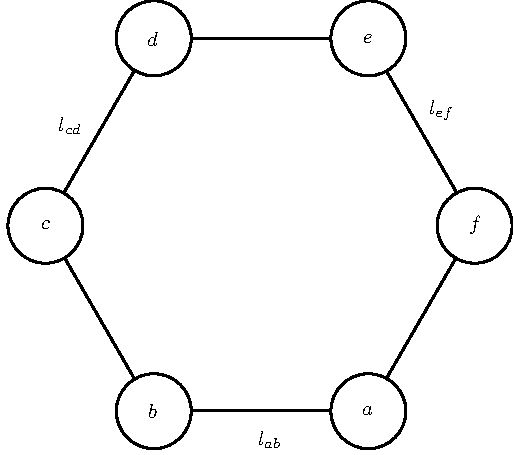
\includegraphics[width=4cm]{circle}
\label{subfiga}}
\hfill
\subfloat[Clique]{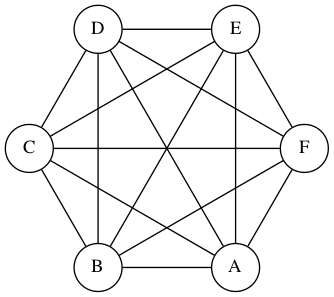
\includegraphics[width=4cm]{clique}
\label{subfigb}}
\caption{Circle and Clique topology of 6 nodes}
\vspace*{0.1in}
\end{figure}


\subsection{Circles}
Cycles topology connect all the nodes by a cycle, any node in which has two links joined. Figure 1 show the six
nodes cycles topology, let nodes named from $A$ to $F$ and links named from $a$ to $f$ in the figure.
Now suppose a traffic in the topology then calculate the optimal routing for it,
let $D_a$ and $C_a$ be the demand and capacity of the link, without loss of generality, we say the link $d$ is the 
bottleneck, i.e. with the maximum link utilization. There are two solutions for us, switching off the link $d$,
or the other link, such as link $f$.


For case one, when we switch off the link $d$, the origin traffic pass the link will be redirected. The worst situation
is that all the traffic on the link $d$ will be put to the other path : $D \leftarrow C \leftarrow B \leftarrow A \leftarrow 
F \leftarrow E$. After traffic redirection, the bottleneck link may become the link $e$, according to our definition of
extended robust link utilization:

\begin{equation}
    \frac {\frac{D_e + D_d} {C_e}} {\frac {D_d}{C_d}} = (1 + \frac{D_e}{D_d}) \frac{C_d}{C_e}
\end{equation}

Because the link utilization of link $d$ is the maximum one, we have :

\begin{equation}
    \frac{D_d}{C_d} > \frac{D_e}{C_e} 
\end{equation}
\begin{equation}
    \frac{D_e * C_d}{C_e * D_d} < 1
\end{equation}

so we have the extended robust link utilization in case one :

\begin{equation}
    (1 + \frac{D_e}{D_d}) \frac{C_d}{C_e} < \frac{C_d}{C_e} + 1
\end{equation}


For case two, similar to case one, all the traffic will be redirected on the other path between $F$ and $A$. There are two 
sub cases after traffic redirection, the link $D$ is still the bottleneck or the link $E$ become the new bottleneck. In sub 
case one:

\begin{equation}
    \frac{\frac{D_d + D_f}{C_d}}{\frac{D_d}{C_d}} = 1 + \frac{D_f}{D_d}
\end{equation}

Because the link utilization of link $d$ is the maximum one in origin topology, we have as:

\begin{equation}
    \frac{D_d}{C_d} > \frac{D_f}{C_f} 
\end{equation}
\begin{equation}
    \frac{D_f}{D_d} < \frac{C_d}{C_f} 
\end{equation}

So we get the extended robust link utilization in this case :
\begin{equation}
    (1 + \frac{D_f}{D_d}) < \frac{C_d}{C_f} + 1
\end{equation}

In sub case two, we get the new extended robust link utilization in link $E$:

\begin{equation}
    \frac{\frac{D_e + D_d}{C_e}}{\frac{D_d}{C_d}} = \frac{D_e * C_d}{D_d * C_e} * \frac{C_d * D_f}{C_e * D_e}
\end{equation}

Similarly as mentioned above, we get equations :

\begin{equation}
    \frac{D_d}{C_d} > \frac{D_e}{C_e} => \frac{D_e * C_d}{C_e * D_d} < 1 
\end{equation}
\begin{equation}
    \frac{D_d}{C_d} > \frac{D_f}{C_f} => \frac{D_f * C_d}{D_d} < C_f
\end{equation}

So we get the extended robust link utilization:

\begin{equation}
    \frac{D_e * C_d}{D_d * C_e} + \frac{C_d * D_f}{C_e * D_d} < 1 + \frac{C_f}{C_e}
\end{equation}

As a result, the upper bound of extended robust link utilization must be :

\begin{equation}
    Max\{1 + \frac{C_d}{C_e}, 1 + \frac{C_d}{C_f}, 1 + \frac{C_f}{C_e}\}
\end{equation}

Particularly, if all the links have the same capacity, the upper bound equal to 2 when switch off one link. Otherwise, the 
upper bound only dependent to the greatest ratio of link capacity.
 
\subsection{Cliques}
In clique topology, all the nodes connect to each other, it means that situation become more difficult because the traffic
can be adjusted to multi paths rather than one path in circle. And we will see that splitting traffic on multi paths is 
always better than put all the traffic to one, so if we get the upper bound of the worst case, it must be the upper bound
of other case. Similarly to circle topology, we say the link $a$ is the bottleneck, and we will switch off it or other link
like $b$.

In case one, after we switch off link $a$, the new bottleneck link must be the affected link, the link contains the origin 
traffic on link $a$. Otherwise if the link $b$ is the bottleneck, but we adjust the traffic on other links, it means that
we can do the same thing in the origin topology, and the bottleneck become link $b$ rather than $a$. It is conflict with our
assumption. So we have the extended robust link utilization as :

\begin{equation}
    \frac {\frac{D_b + D_a}{C_b}}{\frac{D_a}{C_a}} = (1+\frac{D_b}{D_a}) \frac{C_a}{C_b}
\end{equation}

Because the link $a$ is the bottleneck link with the maximum link utilization, like what we do above, we can get 

\begin{equation}
    (1+\frac{D_b}{D_a}) \frac{C_a}{C_b} < 1 + \frac{C_a}{C_b}
\end{equation}

In case two, the bottleneck may still be link $a$ or the new link $c$. If it is link $a$, and no new traffic across it,
the extended robust link utilization equal to 1 obiliously. Or we adjust the new traffic $D_b$ on it, we can get the
extended robust link utilization:

\begin{equation}
    \frac{\frac{D_a + D_b}{C_a}}{\frac{D_a}{C_a}} = 1 + \frac{D_b}{D_a} < 1 + \frac{C_b}{C_a}
\end{equation}

If the bottleneck become new link $c$, similar to our proof of circle topology, we can get extended robust link utilization:
\begin{equation}
    \frac{\frac{D_c + D_b}{C_c}}{\frac{D_a}{C_a}} = \frac{D_c * C_a}{D_a * C_c} + \frac{D_b * C_a}{D_a * C_c} < 1 + \frac{C_b}{C_c}
\end{equation}

So we obtain the same conclusion as circle topology, the extended robust link utilization must be :

\begin{equation}
    Max\{1 + \frac{C_a}{C_b}, 1 + \frac{C_b}{C_a}, 1 + \frac{C_b}{C_c}\}
\end{equation}

\subsection{Other Topology}
We can also see that, when we switch off different link, it really matters the performance which dependent on not only the 
demand or traffic, but also the capacity of links. Particularly, the upper bound is just related with the capacity of links.
And from our proof process, there is no special limitation for specific topology, so we can get the similar conclusion 
on other topology.

\begin{figure*}[!t]
\centering
\vspace*{0.1in}
\subfloat{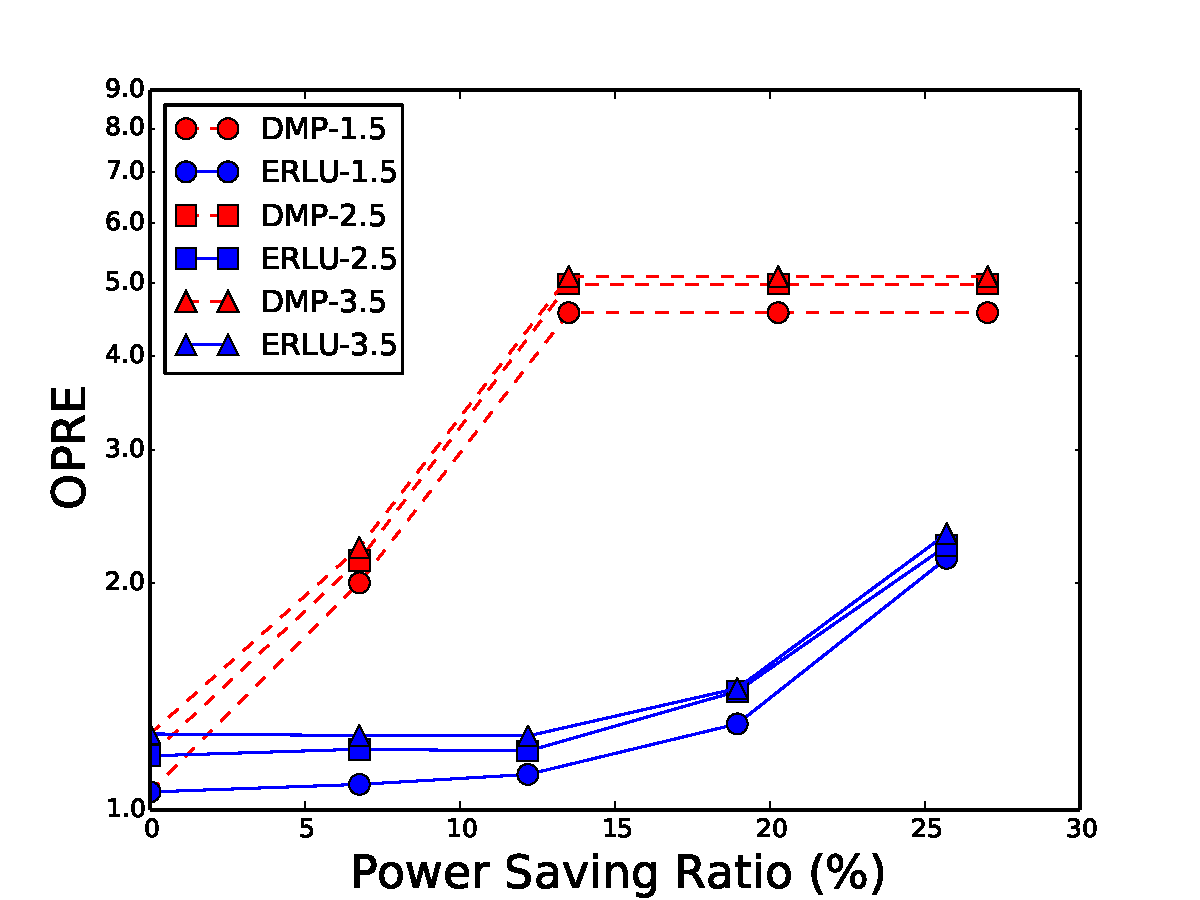
\includegraphics[width=6cm]{opr_with_power_abilene}}
\subfloat{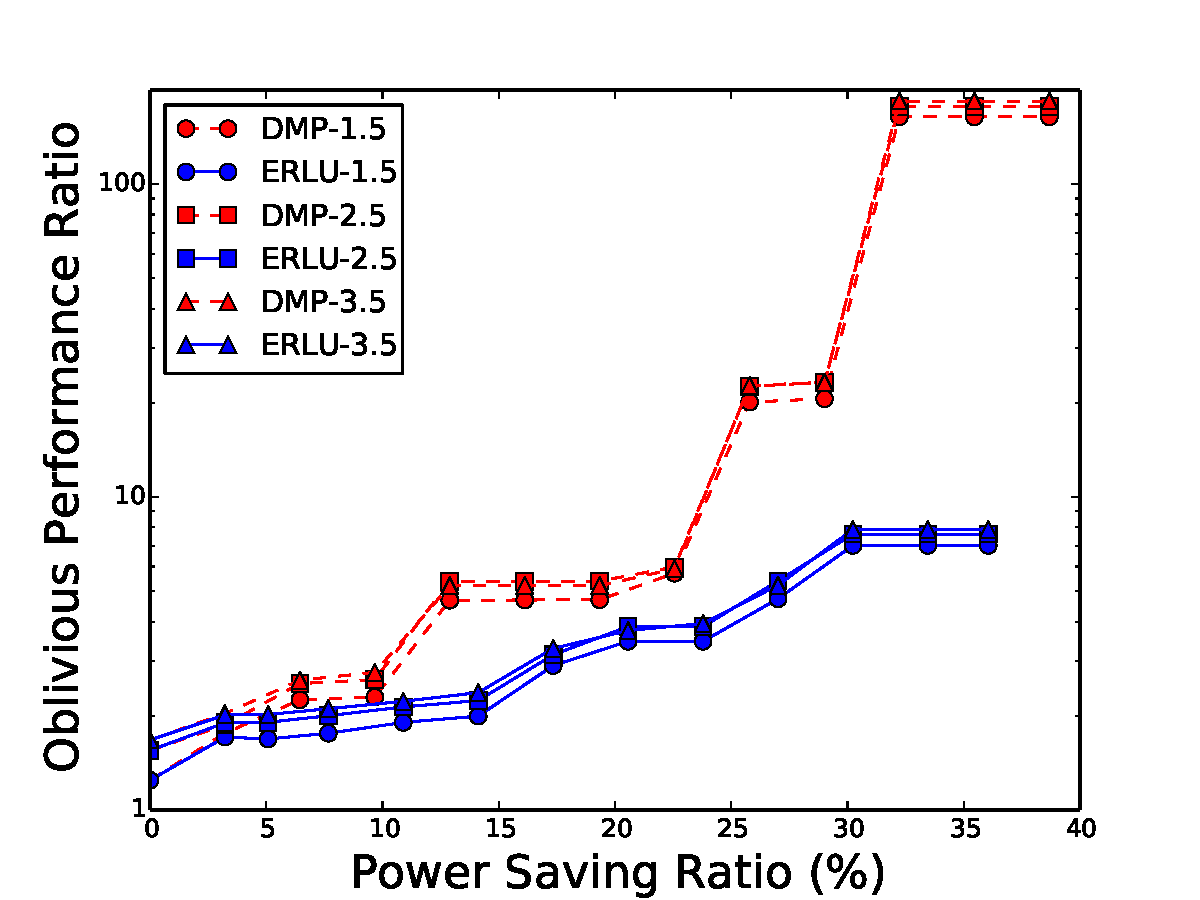
\includegraphics[width=6cm]{opr_with_power_geant}}
\subfloat{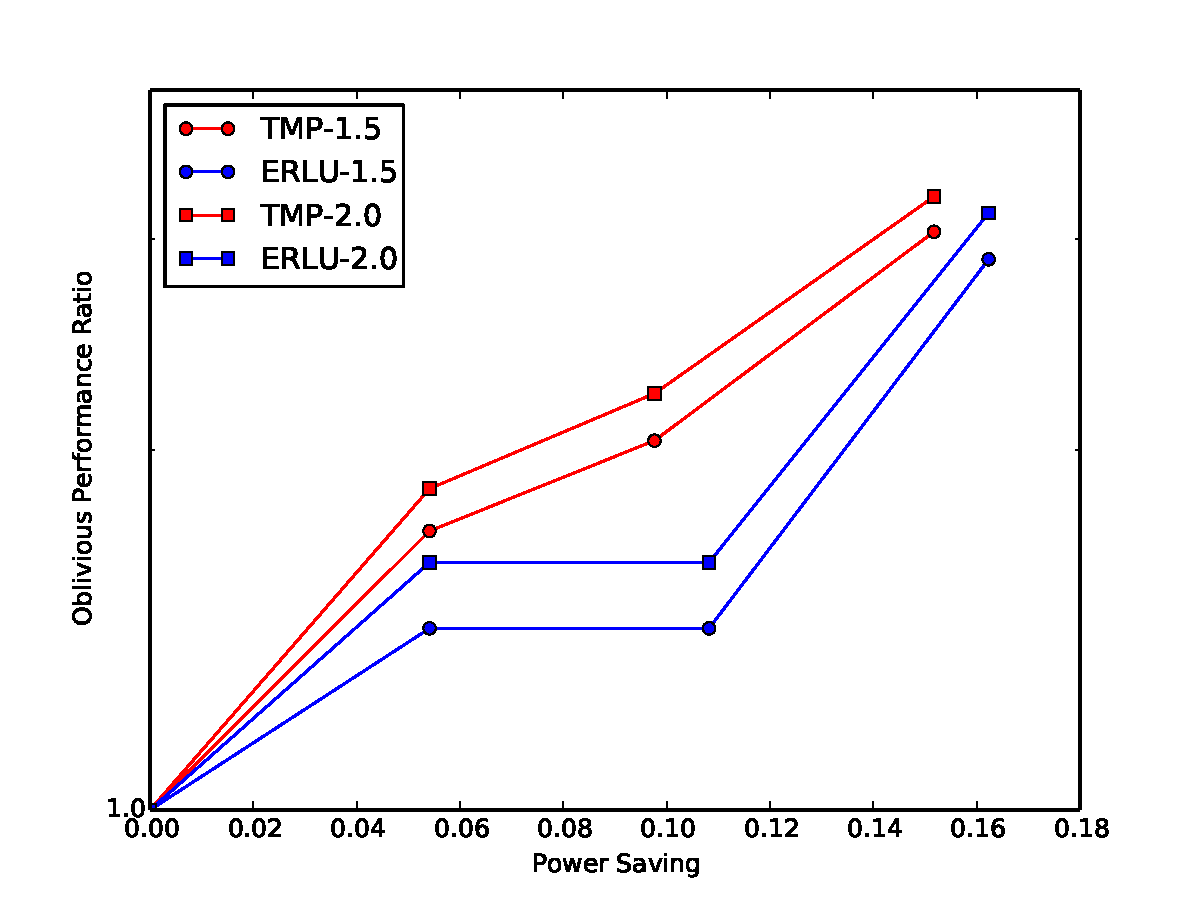
\includegraphics[width=6cm]{opr_with_power_cernet2}}
\caption{OPRE versus Power Saving: (1). Abilene, (b). Geant, (c). Cernet2}
\vspace*{0.1in}
\end{figure*}

\begin{figure*}[!t]
\centering
\vspace*{0.1in}
\subfloat{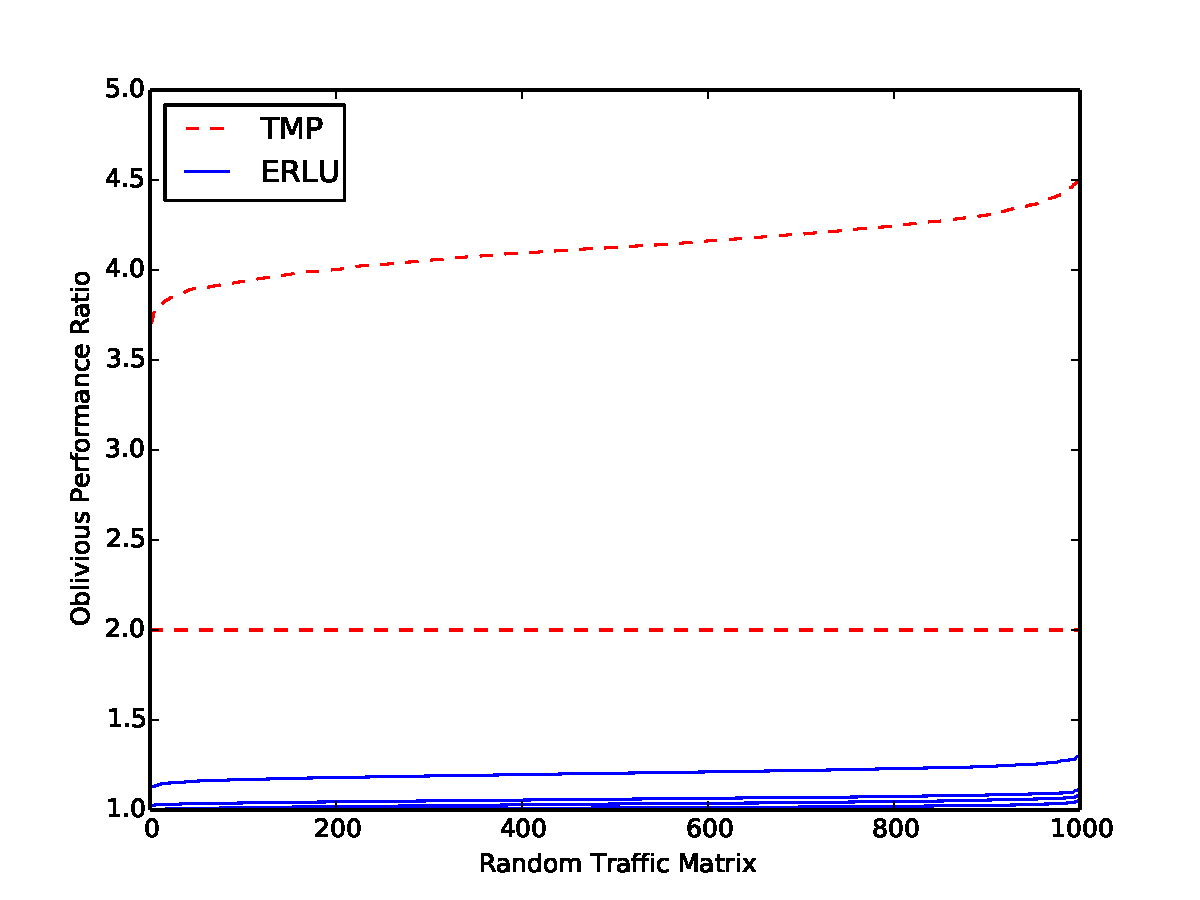
\includegraphics[width=6cm]{exp2_sort_abilene}}
\subfloat{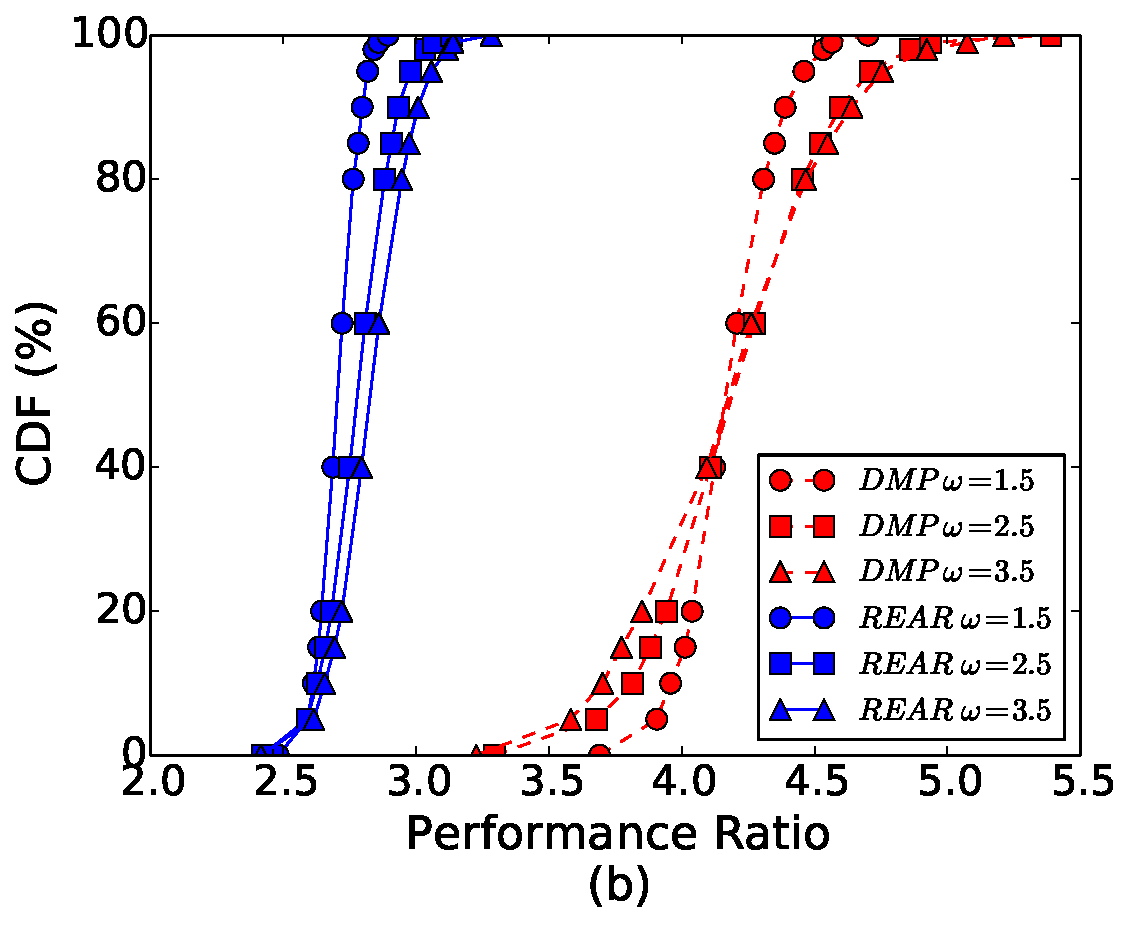
\includegraphics[width=6cm]{exp2_sort_geant}}
\subfloat{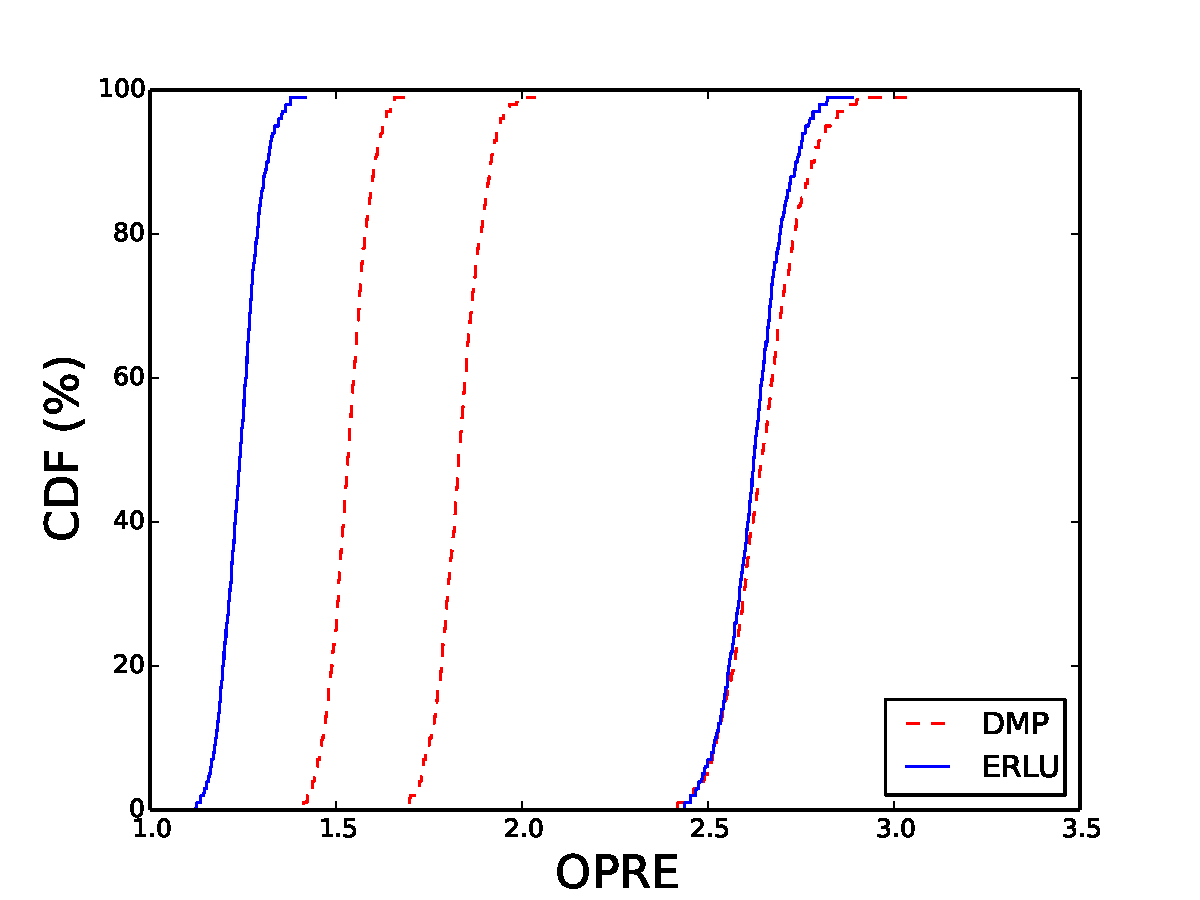
\includegraphics[width=6cm]{exp2_sort_cernet2}}
\caption{OPRE versus TMs: (a). Abilene, (b). Geant, (c). Cernet2}
\vspace*{0.1in}
\end{figure*}


\section{Experiments and Results}
We simulated our algorithm on real world topology, including Abilene, Geant and Cernet2, whose number of nodes and links are listed in Table \Rmnum{1}.
Then we generate random traffic matrix with Gravity Model \cite{networking:gravity}, which assume that the traffic demand between nodes is proportional
to their combined capacity of connecting links. To extrapolate a complete TM, we take an attribute margin $w$ to scale the traffic range from $1/w$ to $w$
base on the basic traffic demand. Particularly, when the $w$ limit extremity, we say the traffic matrix is really arbitrary, and our 
algorithm is irrelevant with traffic.

\begin{table}[!t]
\renewcommand{\arraystretch}{1}
\caption{Topologies}
\label{three topologies}
\centering
\begin{tabular}{|c|c|c|c|}
\hline
\bfseries Topology & \bfseries Nodes & \bfseries Links & \bfseries Links can be Removed \\
\hline
Abilene & 12 & 15 & 4 \\
\hline
Geant & 23 & 37 & 15 \\
\hline
Cernet2 & 20 & 22 & 3 \\
\hline
\end{tabular}
\end{table}


\begin{figure*}[!t]
\centering
\vspace*{0.1in}
\subfloat{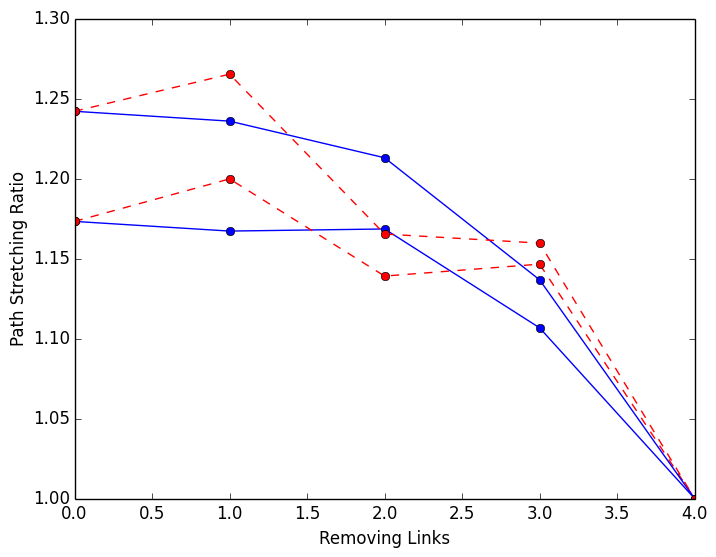
\includegraphics[width=6cm]{exp4_path_abilene}}
\subfloat{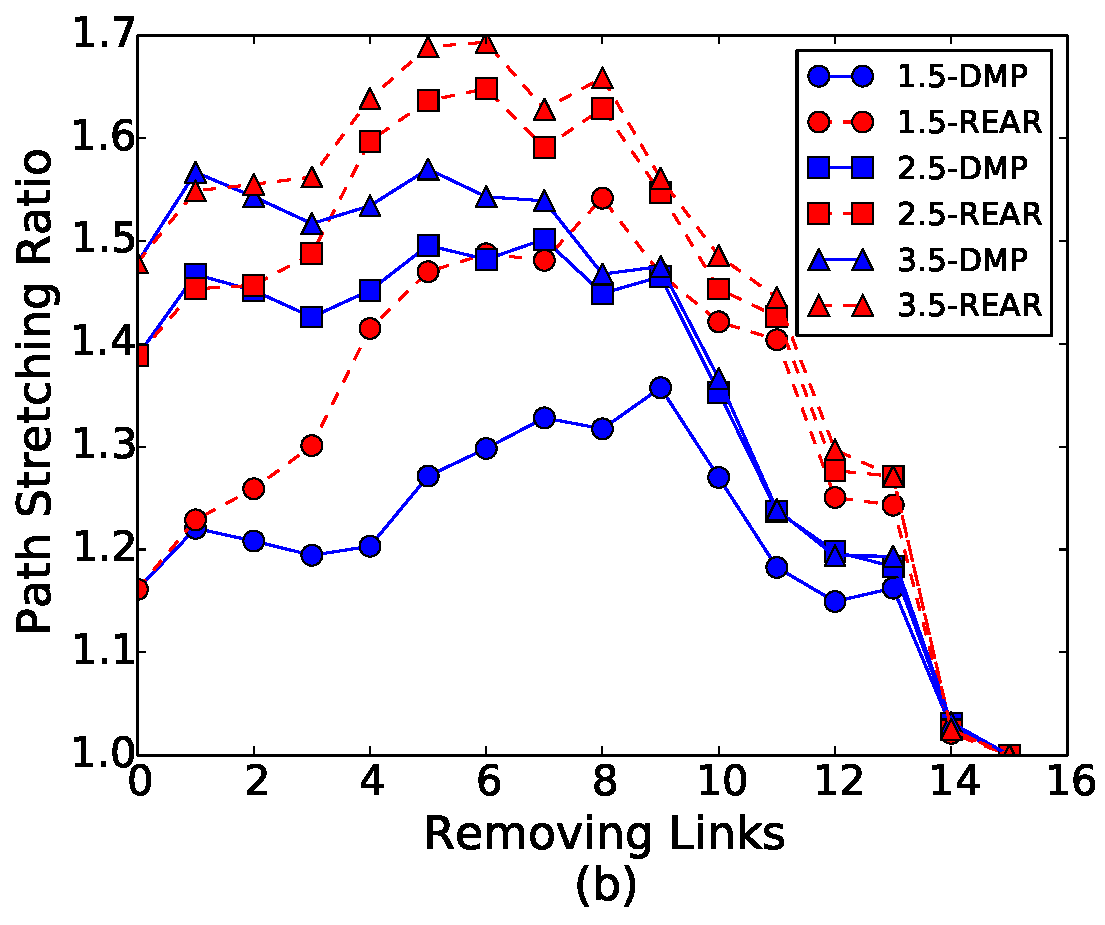
\includegraphics[width=6cm]{exp4_path_geant}}
\subfloat{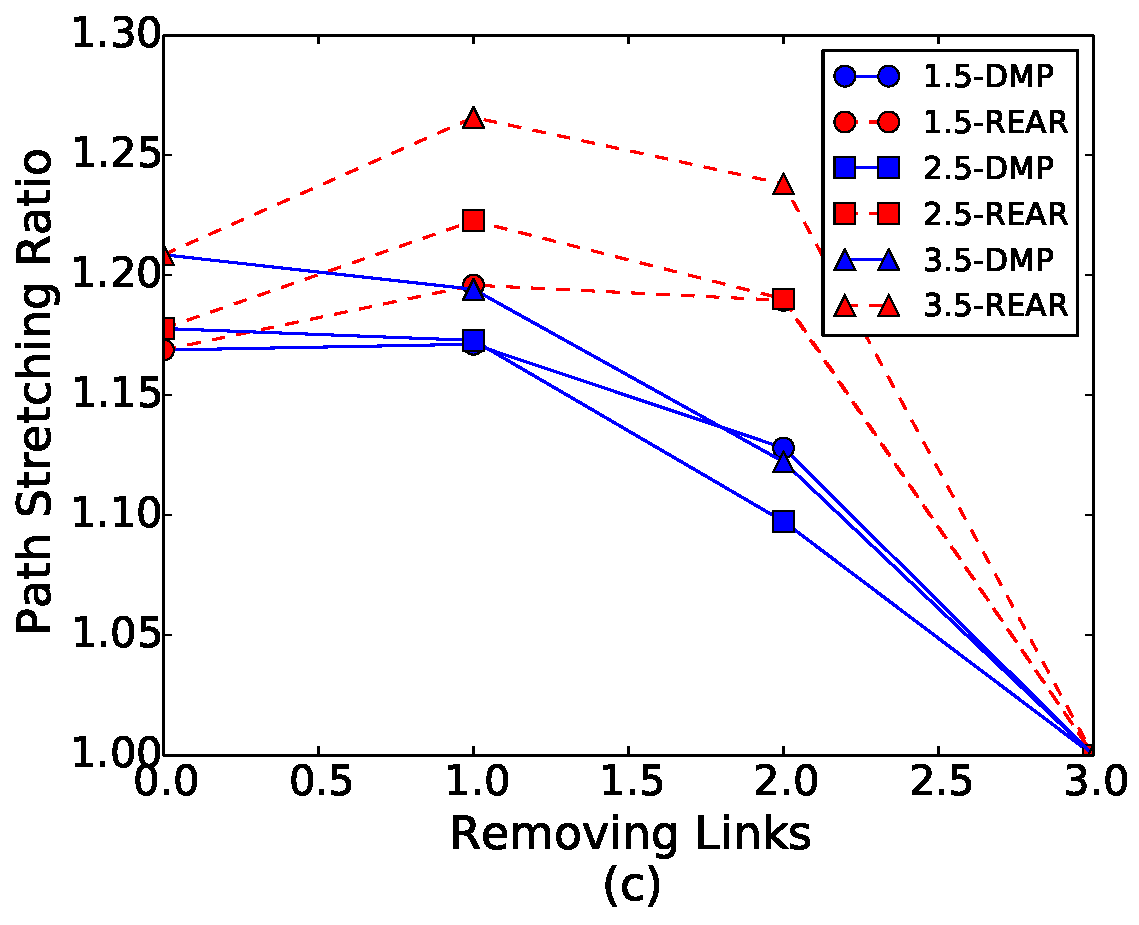
\includegraphics[width=6cm]{exp4_path_cernet2}}
\caption{Path Stretching: (a). Abilene, (b). Geant, (c). Cernet2}
\vspace*{0.1in}
\end{figure*}

\subsection{OPRE versus Power Saving}
In Figure 3, we see that the value of OPRE is at least 1 for all topologies even no links removed, particularly in Geant the value is 1.24,
it means the robust routing always not be the optimal for all TMs. It is reasonable because our robust routing is used for a range of traffic 
rather than a specific TM.


When we switch off links, the topology lose connectivity and some routing paths will be failed, traffic on those paths will be 
adjusted to others, which result in the value of OPRE increased. We take margin from 1.5 to 3.5 and observe this phenomena from Figure.
Pay attention that we scale the y-axis as logarithm for comparing TMP and ERLU in one figure. Intuitively, we can see ERLU is always
better than TMP whatever margin or power saving target is, because ERLU consider much more than TMP, such as capacity and robust traffic 
flows. Another information from Figure 4 is that, we should carefully set the value of power saving for avoiding removing too much
links, which result in the OPRE increases rapidly, induce network congestions easily and make the robust routing be less `robust'.


we concern more about how is the OPRE varifying when achived specific power saving target. Obviously, the more links we removed, 
the more power we saved, but how to quantify the power of one link is difficult. Green TE proposed a simple power model \cite{networking:greente}, 
which can be represented in Table \Rmnum{2}. In which, the total energy of topology is dominant by line cards of routers or switches, 
when saying switch off the links we mean put down the according line cards.

\begin{table}[!t]
\renewcommand{\arraystretch}{1}
\caption{Green TE Power Model}
\label{power model}
\centering
\begin{tabular}{|c|c|c|}
\hline
\bfseries Line-Card & \bfseries Speed(Mbps) & \bfseries Power(Watts) \\
\hline
1-Port OC3 & 155.52 & 60 \\
\hline
8-Port OC3 & 1244.16 & 100 \\
\hline
1-Port OC48 & 2488.32 & 140 \\
\hline
1-Port OC192 & 9953.28 & 174 \\
\hline
\end{tabular}
\end{table}

We compute the power saving ratio as the total power of the removed links over the total power of all the links. 
In Figure 3 (a), it shows we can save 19\% energy only with an OPRE of 1.30 in Abilene topology, and in Geant and Cernet2, 
the OPRE is little higher. Curves present some scalariform, it means that in some range of power saving, the OPRE rise slowly,
and in the end of range, the energy conservation is efficient.


\subsection{OPRE versus Margin}
We take the margin $w$ as one of the input for computing robust routing, and margin identify a range of TMs the routing is 
robust for. Once the $w$ limit extremely, our robust routing is said without knowledge of traffic matrix. Figure 3 shows the 
OPRE increases little as $w$ increases, particularly in Geant, the difference almost can not be observed. It is obvious because
when the $w$ is greater, the traffic matrix is random in more wider range, and our OPRE may achieve worse case with more probability.


\subsection{OPRE versus TMs}
To simulate the worst case, we generate 1000 traffic matrices for every topoloy with margin attribute $w$. Figure 4 shows
the OPRE distribution in the process of experiment. For avoiding mess result from too many lines, we just show the first 
three lines and the base line, which shows the distribution when no links is removed, i.e. seven lines in each figure.


In Figure 4 (a), we can only observe five lines because there are two overlapping lines, which means that when removing 
links the worst case for the robust routing does not change. Maybe the random traffic matrices is not bad enough, or the 
removed link really do not affect the MLUR. And from Figure 4, we see that the OPRE is not always be achived for most
traffic matrices, the common value is much less than OPRE. 


Comparing TMP and ERLU, the conclusion is similar to Figure 3, the latter is always better than the former. Even in some 
time, ERLU obtains more power saving but with a lower OPRE.

\subsection{Path Stretching}
Path stretching must be careful concerned in routing problem. Suppose two vertices connect directly each other in the origin topology,
if we remove the connected link then they can connect by another path which is composed by multi links. However we argue path stretching
between these situation may be unjust, because path stretching result from the difference of topologies rather than routing selection.
So we obtain the shortest path by Dijkstra Algorithm in the final topology, and compare it with robust routings generated by 
our REAR algorithm. Futher, we show the difference between two ways of removing link, and see the tendency when margin increased.

In Figure 5, we see every line ends with path stretching ratio of 1, because topology become a tree structure when lose too much links,
every path between vertices come to be unique, namely each path is the shortest path. Another conclusion is that, even in the origin 
topology, our robust routing is 17\% longer than the shortest one, it is beacuse our algorithm not only consider the MLUR but also 
the robust performance. However the Dijkstra just take the path length as metric.

We can observe that, ERLU is always shorter than TMP, althoungh in Geant, the worst case is 36\% than the shortest path when margin 
equal to 1.5. And in the first removed links, the path stretching ratio is near 20\%. 


\section{Conclusion}
The conclusion goes here.

\begin{thebibliography}{1}

\bibitem{networking:greente}
M.Zhang, C.Yi, B.Liu and B.Zhang, "GreenTE: Power-Aware Traffic Engineering".

\bibitem{networking:oblivious}
D.Applegate and E.Cohen, "Making Intra-Domain Routing Robust to Changing and Uncertain Traffic Demands: Understanding Fundamental Tradeoffs".

\bibitem{networking:gravity}
M.Roughan, A.Greenberg, C.Kalmanek, M.Rumsewicz, J.Yates, and Y.Zhang. Experience in measuring backbone traffic variability: models, metrics, measurements, and meaning. InProceedings of the 2nd Internet Measurement Workshop. ACM, 2002
\end{thebibliography}


% that's all folks
\end{document}



























